\definecolor{exxetagray}{gray}{0.75}
\definecolor{itemcolor}{RGB}{179,217,255}
\definecolor{usercolor}{RGB}{255,204,179}

\shorthandoff{"}
\chapter{Konzeption}
\label{ch:algorithmus}

\section{Gestaltung des Algorithmus}

\subsection{Aggregation}
% Beispielrechnung in Anhang?
% Begründung Auswahl der Kombination der Präferernzen
% Kein harmonisches Mittel, da teilen durch 0 nicht möglich. Da aber MA durchaus fähigkeiten nicht besitzen kommt das häufig vor (man könnte als abhilfe einen Default von 0,000001 setzen o.ä.)
% Berücksichtigung negativer Präferenzen in Anlehnung an: S. 231, file://wsl%24/Ubuntu/home/masc6/Projects/masterarbeit/literatur/recsys%202022%20modeling%20two%20way%20selection%20preference%20for%20person%20job%20fit.pdf

\subsection{Gewichtung}
% Ermitteln der Gewichte: alpha so wählen, dass Endergebnis möglichst optimal -> bedeutet für uns: zufriedene und leistungsfähige Mitarbeiter werden empfohlen -> erscheinen oben im Ranking
% Ziel: Gegeben einer Funktion f, welches von ein oder mehreren Input-Variablen abhängt, finden der Ausprägungen der Input-Variablen, für die f minimal wird. Obacht: f umfasst hier mehr als nur rws, da auch das ranking danach miteinbezogen wird -> zu minimieren ist die Summe der Ränge der zufriedenen und Leistungsfähigen MA über alle Projekte hinweg
% Hier: mithilfe des Brent Algorithmus in anlehnung an die verwandte Arbeit von \textcite[S. 131ff.]{kleinerman:2:inproceedings}
% Nach https://e-maxx.ru/bookz/files/numerical_recipes.pdf S. 489 gibt es keinen perfekten Optimierungs-Algorithmus -> daher ist es grundsätzlih ratsam, verschiedene Techniken auszuprobieren und zu vergleichen.
% Was macht der Brent Algorithmus?: % https://users.wpi.edu/~walker/MA3257/HANDOUTS/brents_algm.pdf

% \begin{itemize}
% 	\item In Essenz einfach eine Strategie für das Finden von lokalen Minima ohne Ableitung, indem sich von einem Intervall iterativ an ein Minima angenähert wird, entweder über GSS oder über SPI % file://wsl%24/Ubuntu/home/masc6/Projects/masterarbeit/literatur/Minimization%20or%20Maximization%20of%20Functions.pdf
% 	\item Unterscheiden zw. Brent Methode für root search und Brent-Methode für Minimasuche ohne Derivate (Ableitung)
% 	\item Kombination von successive parabolic interpolation (schnell) und golden-section search (garantiertes finden von Minimum) % für Erklärung siehe video hier: https://www.youtube.com/watch?v=BQm7uTYC0sg
% \end{itemize}

% Lösung über Python Skript unter Einsatz der scipy-Bibliothek (siehe Anhang).
% minimize_scalar function für das Finden von Minima einer skalaren Funktion (output eines einzelnen Wertes) mit einer Variablen (in unserem Fall alpha), deren default Methode brent ist
% Angeben eines Intervalls (hier: zwischen 0 und 1)
% Beschreibung des Algorithmus in anlehung an file://wsl%24/Ubuntu/home/masc6/Projects/masterarbeit/literatur/Minimization%20or%20Maximization%20of%20Functions.pdf ggf. in den Anhang?

\section{Aufbau des Empfehlungssystems}
% Microservice-Architektur -> Empfehlungs-komponente (Rankings)

% \begin{figure}[H]
%     \centering
% 	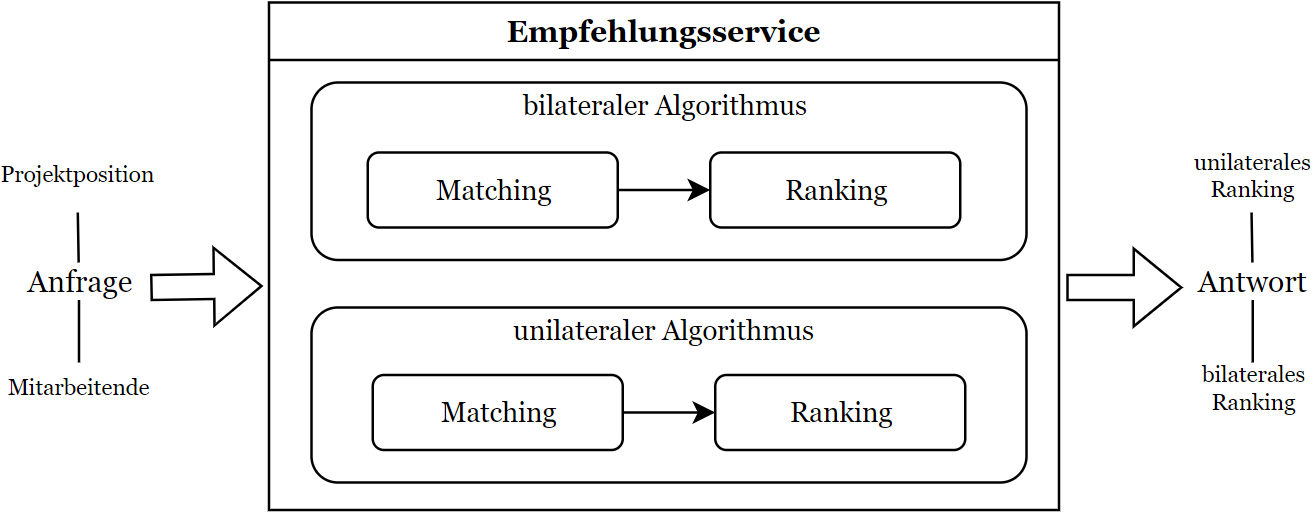
\includegraphics[width=1.0\textwidth]{gfx/empfehlungsservice.png}
% 	\caption[Aufbau des bilateralen Empfehlungssystems]{Aufbau des bilateralen Empfehlungssystems}
% 	\label{fig:algorithmus:abb1}
% \end{figure}

% Begründung für SVR: S: 30, file://wsl%24/Ubuntu/home/masc6/Projects/masterarbeit/literatur/Criteria%20Chains%20A%20Novel%20Multi-Criteria%20Recommendation.pdf

\shorthandon{"}